\documentclass[10pt,titlepage]{article}
\usepackage{fullpage}
\usepackage{graphicx}
\usepackage{float}

\begin{document}
  \title{Lab 6: LabVIEW iRobot Obstacle Avoidance and Hill Climb}
  \author{Sam Mansfield and Toan Vuong \\
          TA: Hoekun Kim \\
          EECS149}
  \date{October 16th, 2013}
  \maketitle

  \section{Introduction}
    In this lab we explored an alternate statechart representation using LabView. By modifying a simple default statechart which navigates an iRobot in a square, we were able to add obstacle avoidance as well as a hill climb algorithm, enabling our robot to climb up a hill despite obstacles being in the way.  

  \section{Analysis}
    % Obstacle avoidance
    Our obstacle avoidance algorithm is essentially that of Lab 4 (Reproduced below), but now implemented in Statechart instead.
    \begin{figure}[H]
        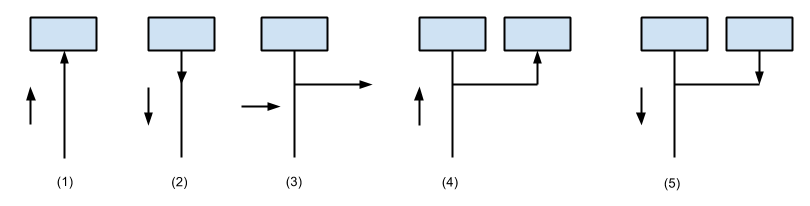
\includegraphics[keepaspectratio, width=1\textwidth]{../lab6_data/a.png}
        \caption{Algorithm Part 1. Single obstacles. Arrows denote direction of travel.}
        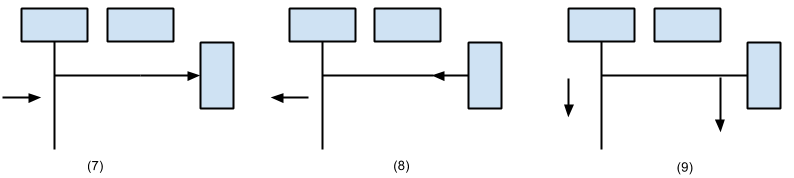
\includegraphics[keepaspectratio, width=1\textwidth]{../lab6_data/b.png}
        \caption{Algorithm Part 2. Encoutering an obstacle while avoiding the first. Arrows denote direction of travel.}
        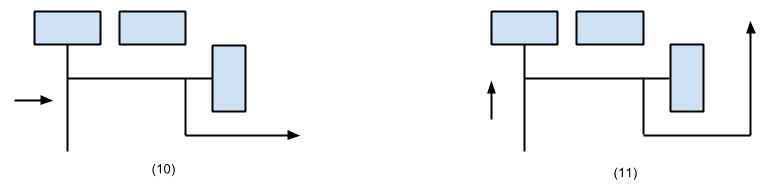
\includegraphics[keepaspectratio, width=1\textwidth]{../lab6_data/c.png}
        \caption{Algorithm Part 3. Recovery from both obstacles. Arrows denote direction of travel..}
    \end{figure}
    It works on the principle that, to avoid an obstacle, we first move backwards to get some room, then we turn. After some time, we assume that the obstacle is no longer in the way, and turn back to our original orientation. If this fails, we continue with the obstacle avoidance algorithm again. 
    \begin{figure}[H]
        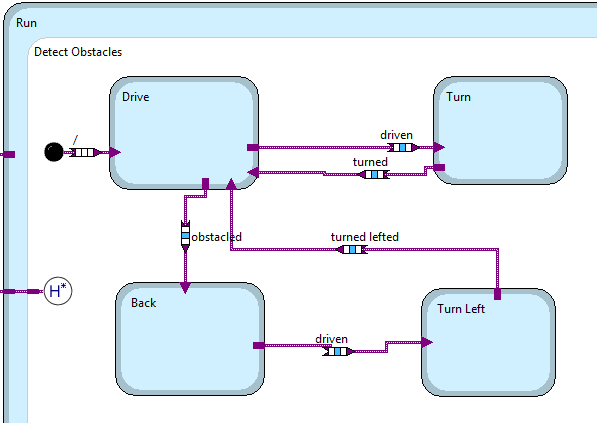
\includegraphics[keepaspectratio, width=0.5\textwidth]{../lab6_data/6_1_SM.PNG}
        \caption{Statechart 1. Obstacle avoidance}
    \end{figure}
    The guards remain the same as they were from Lab 4. We transition to BACK from DRIVE when an obstacle is encoutered. BACK transitions to TURN LEFT after a set distance. TURN LEFT transitions to DRIVE after a set angle. and DRIVE will now transition to TURN after a set distance. This puts us back to our original orientation, and we can transition to DRIVE and continue on our original orientation. We also keep a count of how many turns we've made to account for nested obstacle avoidances.
    
    
    % Hill Climb
    We didn't need to add any states from the obstacle avoidance FSM, but we added several guards. In addition to just detecting hills and climbing them we implemented left and right obstacle detection. Previously we always turned left to go around an object, but Hokeun insisted that we should add the right and left avoidance feature, which we did. Basically when the left sensors pick up an obstacle the number of obstacles are incremented, the robot turns right, and when the robot is back in the original orientation, the number of obstacles are decremented. On the other hand if the right sensors detect an obstacle, the number of obstacles are decremented, the robot turns left, and when the robot is back in the original orientation, the number of obstacles are incremented. 
    The need for this enhancement is justified as follows. If an obstacle is encoutered to the left of the robot, it will turn right to avoid the obstacle. Likewise, if the obstacle is encoutered to the right, it will turn left. This helps with cases where the obstacle is not just in front of the robot, but also to its side or diagonally placed.
    \begin{figure}[H]
        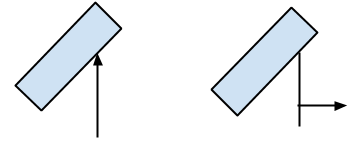
\includegraphics[keepaspectratio, width=0.5\textwidth]{../lab6_data/d.png}
        \caption{Smart turns. The robot will turn in the direction opposite of the obstacle}
    \end{figure}
    Had the robot turned left in Figure 4., it would have encoutered the same obstacle a second time. By using this avoidance scheme and turning opposite of the location of the object, we avoid multiple occurrences of the same obstacle. One subtle factor is the possibility that, given the same number of "left" obstacles and "right" obstacles, our robot can correct for one type of obstacle when encoutering another, avoiding the need to correct for four obstacles (and making a total of 4 turns, instead of 8).

    In order to climb hills, we added two guards. One detects if we are on a hill. In this case we turn the boolean orient to true and rotate until the x axis of the accelerometer is positive (meaning the robot is facing uphill) and the y axis is close to 0 (meaning that the robot is facing directly up the hill). In order to take into account for movement of the robot, we had the robot move very slowly, and it seemed to work quite well. Previously in last lab, we made sure the robot turned a certain amount in order to correct, but this actually caused a lot of problems in simulation.

    \begin{figure}[h]
      \includegraphics[width=\textwidth]{../lab6_data/6_2_SM}
      \caption{State Chart for obstacle avoidance and hill climb.}
    \end{figure}

    Speaking of simulation problems, we had a tremendous amount of trouble in simulation. We got things working in the physical world for the hill climb pretty quickly since we had our algorithm from the previous lab, but we could not use that algorithm in the simulation. At first we thought the accelerometer values were not getting passed correctly to the state chart, but what it turned out to be was the net angle wrapping, which we weren't taking into account. Originally we wanted to have the robot turn at least 45 degrees before trying to detect the top of the hill, and in the real world this works fine, in order to take into account of the movement of the accelerometer. In simulation this did not work, the angle would wrap around so that when the guard was supposed to be true, the net angle had wrapped and now the guard was no longer true, so our robot was orienting continuously and never went up the hill.

    The differences between simulation and the real world mainly had to do with magic numbers. For instance in the simulation we might use something like when z is less than 0.99, but in the real world when z is less than 0.9 is a more reasonable value. Another differences is that in the simulation 90 degrees means 90 degrees, but in the physical world 90 degrees is more like 73 net angle degrees. It only came down to magic numbers that make the robot transition smoother.

    Considering how robust LabVIEW is, we were not able to easily debug our program, we couldn't figure out how the probe tool worked, and considering that in the real world our algorithm worked it was intensely frustrating for the simulation to continuously not work without being able to find out why. As much as LabView pretends to be a friendly environment it is much easier for us to write and debug the robot in C than it was in LabVIEW. In short, Statecharts with LabView is a great idea, but requires a lot of further refinement if it wants to be of use. As it stands, it is much easier to translate our model to C.

    One other source of annoyance is the amount of errors we received in LabView. Deploys to our robot would take up to 5 tries, failing due to some memory error. We found out that we needed to "Force code generation" before we deploy, despite not having changed anything since the last generation. Without doing this, the deploy would crash.

  \section{Conclusion}
    In this lab we learned how to use LabView state charts to design an algorithm to avoid obstacles and climb hills. We learned about the simulation capabilities and structure that can be used to create projects in LabView. 
\end{document}
